    %! Author = Omar Iskandarani
    %! Title = VAM: Explaining the Universe in Analogies
    %! Date = xx-xx-2025
    %! Affiliation = Independent Researcher, Groningen, The Netherlands
    %! License = © 2025 Omar Iskandarani. All rights reserved. This manuscript is made available for academic reading and citation only. No republication, redistribution, or derivative works are permitted without explicit written permission from the author. Contact: info@omariskandarani.com
    %! ORCID = 0009-0006-1686-3961
    %! DOI = 10.5281/zenodo.xxxxxxx

% === Metadata ===
    \newcommand{\papertitle}{VAM: Explaining the Universe in Analogies}
    \newcommand{\paperdoi}{10.5281/zenodo.xxxxxxxx}


    \documentclass[a4paper,12pt]{article}
    \usepackage{../vamstyle}

    \usepackage{import}
    \usepackage{subfiles}
    \pgfplotsset{compat=newest}
    \usepgfplotslibrary{patchplots}

\usepackage[unicode]{hyperref}
\hypersetup{pageanchor=false}
    \usepackage{caption}


    % vamappendixsetup.sty

\newcommand{\titlepageOpen}{
  \begin{titlepage}
  \thispagestyle{empty}
  \centering
  {\Huge\bfseries \papertitle \par}
  \vspace{1cm}
  {\Large\itshape\textbf{Omar Iskandarani}\textsuperscript{\textbf{*}} \par}
  \vspace{0.5cm}
  {\large \today \par}
  \vspace{0.5cm}
}

% here comes abstract
\newcommand{\titlepageClose}{
  \vfill
  \null
  \begin{picture}(0,0)
  % Adjust position: (x,y) = (left, bottom)
  \put(-200,-40){  % Shift 75pt left, 40pt down
    \begin{minipage}[b]{0.7\textwidth}
    \footnotesize % One step bigger than \tiny
    \renewcommand{\arraystretch}{1.0}
    \noindent\rule{\textwidth}{0.4pt} \\[0.5em]  % ← horizontal line
    \textsuperscript{\textbf{*}}Independent Researcher, Groningen, The Netherlands \\
    Email: \texttt{info@omariskandarani.com} \\
    ORCID: \texttt{\href{https://orcid.org/0009-0006-1686-3961}{0009-0006-1686-3961}} \\
    DOI: \href{https://doi.org/\paperdoi}{\paperdoi} \\
    License: CC-BY 4.0 International \\
    \end{minipage}
  }
  \end{picture}
  \end{titlepage}
}
    \begin{document}

        % === Title page ===
        \titlepageOpen



        \begin{abstract}

            This guide provides an accessible, richly illustrated introduction to the Vortex Æther Model (VAM)—a novel framework in physics that reimagines the fabric of reality as a vast, dynamic ocean of superfluid æther. Unlike conventional theories that describe gravity as the bending of spacetime or particles as indivisible points, VAM envisions all matter, energy, and even time itself as emergent from swirling knots, loops, and flows within this universal fluid.

            Designed for curious laypeople, students, and interdisciplinary thinkers, each section replaces daunting equations with engaging analogies. Readers are invited to picture the universe as a calm pond where every particle is a smoke ring, every force a current, and every moment a ripple on the surface. The guide journeys from ancient philosophical notions of æther through the visions of Maxwell, Kelvin, and Einstein, and into the VAM’s modern reinterpretation—making connections with contemporary fluid dynamics and recent experiments with knotted vortices.

            Illustrations and sidebars reinforce each metaphor:

            \begin{itemize}
                \item             Particles become knots and whirlpools, with mass arising from their swirl energy and chirality.
                \item             Gravity emerges as a cosmic pressure gradient, like leaves drifting into a whirlpool, not as a mysterious force or spacetime curvature.
                \item             Time is reimagined as both an absolute background rhythm and a local “swirl clock” within each knot, revealing layered and relative tempos throughout the universe.
                \item             Electromagnetism, dark matter, and even the structure of galaxies are explored as patterns of flow and connectivity in the ætheric sea.
            \end{itemize}

            The guide contrasts VAM’s perspective with that of General Relativity and Quantum Mechanics, highlighting how shifting from geometry to flow can open new ways of thinking—and new possibilities for experiment and discovery. Above all, this work demonstrates the transformative power of analogies: not only as learning tools, but as springboards for imagination, insight, and the next generation of scientific breakthroughs.

        \end{abstract}


        \titlepageClose

        \ifdefined\standalonechapter
        \section{\papertitle}
        \else
        \fi
% ============= BEGIN of content ============

        \tableofcontents
        \newpage

%        \begin{tikzpicture}
%  \begin{axis}[
%    view={45}{35},
%    axis lines=none,
%    ticks=none,
%    colormap/cool,
%    samples=200,
%    domain=0:6.2832,  % 0 to 2π
%    z buffer=sort,
%    ]
%    \addplot3 [
%      thick,
%      black,
%      samples=200,
%      domain=0:6.2832,
%    ]
%    ( {0.1015*cos(deg(x)) + 0.063367*sin(deg(x)) - 0.058576*cos(deg(3*x)) - 0.047834*sin(deg(3*x) +  0.010809*cos(deg(5*x)) - 0.123037*sin(deg(5*x)) - 0.019292*cos(deg(7*x)) + 0.002397*sin(deg(7*x)) + 0.021062*cos(deg(9*x)) - 0.027679*sin(deg(9*x))}, {-0.360746*cos(deg(2*x)) - 0.006923*sin(deg(2*x)) + 0.008628*cos(deg(4*x)) - 0.021589*sin(deg(4*x)) - 0.044936*cos(deg(6*x)) + 0.021844*sin(deg(6*x)) - 0.003736*cos(deg(8*x)) - 0.004946*sin(deg(8*x)) - 0.001866*cos(deg(10*x)) + 0.020238*sin(deg(10*x))}, {0.018163*cos(deg(x)) - 0.01601*sin(deg(x))+ 0.050709*cos(deg(3*x)) - 0.083507*sin(deg(3*x)) + 0.101439*cos(deg(5*x)) - 0.013338*sin(deg(5*x)) - 0.040565*cos(deg(7*x)) - 0.010632*sin(deg(7*x)) - 0.00138*cos(deg(9*x)) + 0.021509*sin(deg(9*x))});
%  \end{axis}
%\end{tikzpicture}

        

\section{Introduction: Why Analogies?}

Physics often hides behind walls of equations, intimidating even the most curious minds. But at its heart, every truly profound idea in science first appears as a vivid mental image—a moving story, a metaphor, or even a game of imagination. When we talk about space, time, and matter, it’s easy to get lost in the math. Yet, the greatest breakthroughs often began with analogies: Einstein imagining himself riding on a beam of light, Faraday picturing lines of force in the air, or Newton thinking of an apple falling from a tree.


The Vortex Æther Model (VAM) is no different. It asks us to step beyond traditional ways of thinking—beyond the abstract geometry of General Relativity or the ghostly probabilities of Quantum Mechanics—and instead to imagine the universe as a single, endless ocean: a superfluid æther, whose hidden currents, knots, and waves create everything we see and feel.


Why use analogies? Because they allow us to grasp the core of a new idea before we ever need numbers. They let us “see” how things work, even if those things are too tiny, too fast, or too strange to observe directly. In VAM, this approach is especially helpful, because its concepts are both new and deeply intuitive—if we allow ourselves to picture them.


Goal:

To show how mass, gravity, and time emerge not from mysterious “spacetime” or abstract fields, but from the swirling structure and energetic patterns of a universal superfluid. To reveal how nature’s most fundamental behaviors might all arise from the way the æther moves, swirls, and ties itself into knots.


Method:

We’ll use everyday analogies—calm ponds, rushing rivers, twisting knots, swirling storms, and dancing whirlpools—to bring the vision of VAM to life. Our aim isn’t to avoid the mathematics forever, but to build intuition first, so that the technical details, when encountered, make sense at a gut level.


The invitation:

Let your imagination swim. We’re going to explore a universe where the tiniest particles are miniature whirlpools, where gravity is the current pulling objects along, and where time itself flows differently depending on how wild the local waters become.
        
\section{What is the Æther?}

Imagine you’re standing by a perfectly still pond on a windless day. The water is so calm it’s like a giant mirror, stretching as far as you can see. Now, imagine that this pond isn’t just a body of water in a park, but instead fills all of space—there’s no edge, no bottom, no islands, just water everywhere. This is the kind of universal “pond” that physicists once called the æther.


The æther isn’t just a modern sci-fi idea. It traces its roots through some of the greatest scientific and philosophical minds in history:


\begin{itemize}

\item
Plato \& Socrates spoke of a cosmic "substance" and universal time—an underlying order that everything participates in, whether or not it can be seen.




\item
Isaac Newton imagined an absolute space and time, an invisible arena for all physical action.




\item
James Clerk Maxwell crafted the equations of electromagnetism while picturing invisible gears and vortices in a mechanical æther, weaving the dance of light and magnetism into this medium.




\item
Lord Kelvin (William Thomson) believed atoms themselves were stable knots or loops of motion in the æther—like smoke rings that never unravel.




\item
Hermann von Helmholtz showed that vortex rings in a fluid have remarkable stability, inspiring visions of particles as topological defects in an endless medium.




\item
Even Einstein began his career surrounded by debates about the æther, and his revolutionary 1905 theory of special relativity made the classical, light-carrying æther unnecessary. He did not actually write “the æther does not exist” (a common misconception). Instead, he wrote:



"The introduction of a 'luminiferous æther' will prove to be superfluous inasmuch as the view here to be developed will not require an 'absolutely stationary space' provided with special properties..."

Yet, Einstein’s view continued to evolve. By 1920, he clarified:

"More careful reflection teaches us, however, that the special theory of relativity does not compel us to deny æther. We may assume the existence of an æther; only we must give up ascribing a definite state of motion to it, i.e., we must abstain from talking about the movement of æther."

And in his famous Leiden lecture, he boldly stated:

“According to the general theory of relativity, space is endowed with physical qualities; in this sense, therefore, there exists an æther. ...space without æther is unthinkable.”





\end{itemize}

For centuries, scientists pictured the æther as an invisible medium that carried light, much like air carries sound. In the late 1800s, experiments failed to detect this mysterious substance, and the æther was declared obsolete. But the Vortex Æther Model (VAM) brings the idea back with a radical upgrade: the æther isn’t a “stuff” in space, it is space. It’s not made of atoms or particles, but is more like a superfluid—think of liquid helium cooled so far it flows without friction, or a perfectly coordinated crowd moving as one.


In VAM, this æther isn’t a relic—it’s a real, perfectly smooth, frictionless fluid that fills all of space, a living superfluid sea. Instead of being passive, it’s dynamic and creative: when it swirls, ripples, or ties itself into knots, it gives birth to everything from light to gravity to time itself. All the action in the universe—light, gravity, matter, time—happens because of how this fluid moves, swirls, and forms patterns. The æther is the stage, the actor, and the script all at once. Instead of being a silent, invisible backdrop, it’s the main player in the story of reality.


Sidebar: Æther, Old and New


\begin{itemize}

\item
\textit{Old æther}: A mechanical medium, like invisible air for light waves—eventually disproven by experiment.




\item
\textit{Einstein’s geometric æther}: Not mechanical, but “endowed with qualities”—it bends, stretches, and curves.




\item
\textit{VAM æther}: Like a perfect superfluid pond. All of reality is the dance of this invisible water—knots and swirls in this ocean are what we experience as matter and force.




\end{itemize}

If you could swim through this æther, you wouldn’t feel resistance. But, like a fish sensing the currents, you could “feel” the patterns—vortices, knots, and ripples—that make up everything from atoms to galaxies. In VAM, the æther is not just a scientific guess—it’s the deep water in which all the universe’s mysteries unfold. Every particle, every force, every second that ticks by is really the pattern of swirls, knots, and flows in this infinite, invisible ocean.
        
\section{Particles: Knots and Whirlpools in the Fluid}

If the æther is an endless, invisible ocean, then what are particles—electrons, protons, atoms? In the Vortex Æther Model, they are not tiny balls or indivisible points. Instead, they are knots, loops, and whirlpools formed in the æther itself.


\subsection*{Smoke Rings, Whirlpools, and Knots}

\begin{itemize}

\item
Smoke rings: Imagine blowing a smoke ring across a room. The ring keeps its shape, moving steadily through the air, even as the smoke particles slowly drift away. Its stability comes not from what it’s made of, but from the pattern of swirling motion. In VAM, an electron or a proton is like a cosmic smoke ring, a swirling knot that can travel long distances while staying intact.




\item
Whirlpools in water: Drop a stick into a slow-moving stream. Watch the little whirlpools that form and persist. In VAM, every particle is a miniature whirlpool—a stable pattern, not a thing. Scientists can actually create “vortex knots” in water using clever experimental setups, tying the fluid itself into trefoil shapes that swim through the tank, demonstrating how such knots can be both real and robust.




\item
Knots in rope: Take a piece of string and tie a knot. No matter how you twist the rope, the knot keeps its identity—unless you untie it. In the æther, certain knots are impossible to untie without breaking the underlying “rope” of the fluid. Each type of knot corresponds to a different particle.




\end{itemize}

\subsection*{From Ancient Atoms to Modern Vortices}

For centuries, atoms were imagined as indivisible, solid building blocks. But in VAM, particles are more like patterns or structures—topological “defects” in the ocean of æther. Each knot has its own shape and complexity, which determines what kind of particle it is:


\begin{itemize}

\item
A simple loop might be a photon.




\item
A trefoil knot—a three-lobed, chiral twist—might be an electron.




\item
More complex knots form protons, neutrons, or heavier particles.




\end{itemize}

\subsection*{Water Tank and Trefoil Knot Experiments}

In recent years, physicists have shown it’s possible to tie real knots in water using carefully shaped 3D-printed wings, creating moving trefoils and other vortex knots. These knots persist and travel, proving that the laws of fluid dynamics allow knotted “particles” to exist in a tangible way—even in a simple tank of water. The VAM model is inspired by these findings, taking the idea further: in the æther, every particle is a kind of enduring, swirling knot, much like those seen in the laboratory.


\subsection*{Why Are These Patterns Stable?}

One of the most surprising features of these knots is that they form invisible, nearly spherical boundaries—almost like an imaginary bubble—around themselves. Inside this boundary, the swirling motion balances the pressure with the surrounding æther, creating a zone of perfect equilibrium. This means that a vortex knot, though it looks wild and tangled on the inside, is actually gently “cushioned” against its environment, held together by equal pressure pushing in from all sides. Just as a soap bubble’s surface balances the air inside and outside, so does each æther knot find a stable, roundish edge within the fluid.

Just as a smoke ring or whirlpool resists being broken apart by the water or air around it, vortex knots in the æther are held together by the laws of fluid motion. These rules (discovered by Helmholtz and others) ensure that certain knots are incredibly stable—they can persist for billions of years unless disturbed by something truly powerful.


\subsection*{The Universe as a Sea of Knots}

So, in VAM, the universe is not built from tiny billiard balls, but from persistent knots and whirlpools—subtle, organized dances in the ever-moving æther. Everything, from light to matter, is a kind of swirl, a twist, or a loop in the great cosmic sea.


Analogy Bite:


\begin{itemize}

\item
“If all of space is a pond, then a particle is like a smoke ring under water—a twist in the flow that gives it identity, energy, and even charge.”




\end{itemize}
        
\section{The Swirl of Gravity and Mass: VAM’s Fluid Universe}

How does gravity work in a universe made of fluid and knots? In the Vortex Æther Model (VAM), gravity isn’t a mysterious pulling force, nor is it the bending of a spacetime “fabric.” Instead, it’s all about pressure and swirl—just like the familiar world of water and air.


\subsection*{The Swirl-Pressure Analogy}

Imagine stirring a spoon in a cup of tea. As the liquid swirls, you’ll notice that bits of tea leaves drift toward the center—not because they are being “pulled,” but because the swirling motion lowers the pressure at the center. The faster the swirl, the lower the pressure, and the stronger the inward drift.


\subsection*{Gravity as the Pressure Drop from Swirling Æther}

In VAM, every massive object—whether a particle, planet, or star—is just a big, energetic swirl or knot in the æther. The rapid motion inside the knot creates a pressure drop at its core. Other knots (or “particles”) feel this pressure difference and are swept inward, much like tea leaves spiraling toward the middle of a cup.


No “Force,” Just Flow:


\begin{itemize}

\item
In everyday life, we often talk about gravity as a force pulling things down. In VAM, it’s more accurate to think of things as being swept along by the pressure gradients of swirling æther, not pulled by some invisible hand.




\end{itemize}

\subsection*{Bernoulli’s Law: The Key to VAM Gravity}

Physicists have long known that faster-moving fluids create lower pressure—a principle called Bernoulli’s Law. VAM uses this idea on a cosmic scale: where the æther swirls fastest, the pressure is lowest. This is why massive objects “attract” each other—they are drawn into each other’s low-pressure, high-swirl zones.


\subsection*{Mass as Stored Swirl Energy and the Role of Chirality}

In VAM, there’s another crucial ingredient: chirality, or handedness. This isn’t just a left-vs-right property—chirality is what gives a vortex knot its “spin” and sense of direction through time. Each knot in the æther seeds an internal swirl-thread, an axis along which its spin points and evolves—a bit like the axle of a spinning top threading forward through the fluid.


This swirl-thread is more than just a feature; it’s what creates both mass and time for the particle. The internal “twistiness” (helicity) stores energy and sets the knot’s alignment with the flow of æther time. Mass emerges because the knot’s swirl and twist create pressure and energy in the æther. The direction in which the swirl-thread points determines how the knot experiences time, giving particles their arrow of evolution.


A knot’s mass isn’t just the amount of swirl—it’s the \textit{chirality} and \textit{helicity} of that swirl that bring the knot to life, giving it energy, direction, and its own tiny clock inside the universe’s fluid. What we call “mass” is simply the energy locked into a vortex knot—the faster and tighter the swirl, the greater the pressure drop, and the more massive the particle appears. The knot doesn’t have mass because it is made of something heavy, but because it traps energy in its spinning motion.


\subsection*{The Corkscrew Thread: Building the Fabric of Space and Time}
\begin{figure}[H]
    \centering
    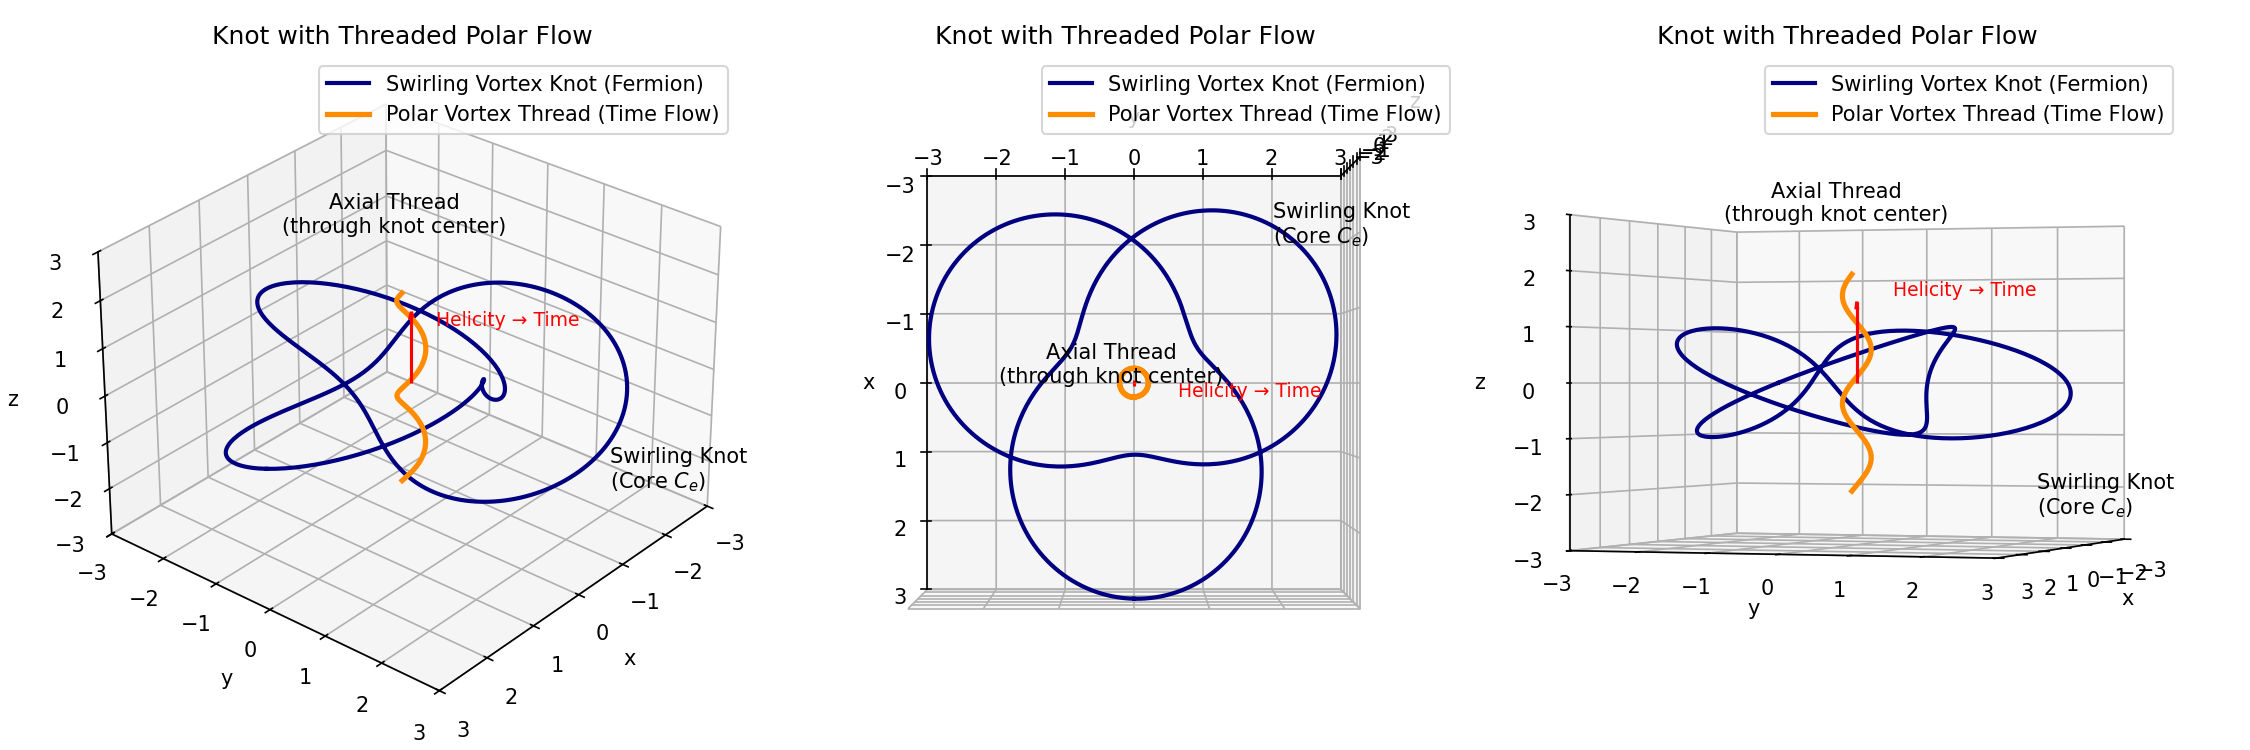
\includegraphics[width=0.7\textwidth]{KnotThreadedPolarFlow}
    \caption{The corkscrew thread inside a vortex knot, showing how particles “thread” their own direction through the æther.}
\end{figure}

Imagine looking inside a vortex knot in the æther: at its heart runs a swirling, corkscrew-like thread. This is more than just the “spin axis” of the knot—it’s the knot’s lifeline, threading its way along the flow of time itself.


\begin{itemize}

\item
This thread—the axial swirl-thread—acts as a kind of backbone. Its direction gives the knot not just its chirality, but also its unique “arrow of time.” The way it twists and moves tells the knot how to evolve, much like a screw turning through wood.




\item
In the VAM universe, these threads don’t stay isolated. As knots form and move, their internal time-threads can reach out, weaving together with others. Over vast distances—perhaps lightyears—these interconnected threads help create the fabric of reality itself: a giant network of twisted, swirling “roads” that structure both space and time.




\end{itemize}

Just as a tapestry is woven from countless threads, the universe’s structure is built from the interconnected time-threads of swirling vortex knots. The chirality at each core is the source of both mass and the local direction of time, while the threads themselves stretch out, forming the backbone of space’s grand design.


\textit{See the illustration: the orange corkscrew thread inside the blue knot shows how each particle “threads” its own direction through the cosmic æther. These threads may connect across enormous distances, helping to shape the entire universe’s flow of space and time.}



\subsection*{Bolts, Nuts, and the Cosmic Pressure Map}

Picture each swirl-thread in a particle as a bolt—a twisting screw that not only keeps the knot together but also creates a line of motion through the æther, like drilling through space. Every knot is like a nut, perfectly shaped for its bolt. As these bolts (swirl-threads) turn, they carve out lines of lowest pressure in the surrounding fluid.


\begin{itemize}

\item
Each bolt (swirl) acts as a channel of lowest pressure. Where there are more bolts in a region—say, at the heart of the Sun—the pressure drops further and further, just like the eye of a whirlpool.




\item
If you could map all the bolts (swirl-threads) radiating out from a star or nucleus, you’d see something like a child’s drawing of the sun: dense beams shooting out from the center, thinning as you move away. The highest density of bolts is at the sun’s center, and the farther you go, the fewer the bolts, and the weaker the pressure drop.




\item
In VAM, each quark contributes one bolt—so more quarks mean more swirl-threads, more lines of low pressure, and a deeper gravitational “well.”




\end{itemize}

\subsubsection*{What about antimatter?}

Antimatter is like a bolt with mirrored threads—spinning in the opposite direction compared to ordinary matter. But in VAM, mirrored bolts still create their own pressure drops: antimatter contributes to gravity just as matter does. The difference is in their internal time and chirality, not in their ability to swirl the æther and create gravitational wells.


In summary: Both matter and antimatter bolts deepen the cosmic “pressure map.” Wherever you find more swirling bolts, you find lower pressure, stronger gravity, and a brighter “beam” in the universe’s great tapestry.



\section*{Analogy Bite}

\begin{itemize}

\item
“Gravity is like the way leaves drift toward a whirlpool in a pond—not because they are pulled, but because they follow the gentle push of water toward the center, where pressure is lowest and the swirl is strongest.”




\end{itemize}
        
\section{Time: Absolute, Local, and Swirl Clocks}

What is time in the Vortex Æther Model? Unlike our everyday clocks or even the “spacetime” of Einstein’s relativity, VAM introduces a new way to think about time—as both an ever-present background rhythm and a local beat set by the motion of knots and swirls.


\subsection*{Universal Time: The Background Music}

Imagine a vast concert hall where a gentle, perfect rhythm plays in the background—so steady that everyone can agree on its tempo. This is absolute æther time in VAM: a universal “metronome” ticking everywhere at once, providing the stage on which all cosmic dances take place. All events unfold within this ongoing, never-skipping background time.


\subsection*{Local Time: The Dancer’s Tempo}

But step onto the dance floor (inside a knot or near a swirling vortex), and something changes. Each dancer—each particle—moves to their own tempo, sometimes slower or faster than the background beat, depending on how wild their local swirl is. This is local (proper) time: inside a rapidly swirling knot, the clock ticks more slowly compared to the calm of the æther ocean. The wilder the local dance, the slower time moves for that dancer.


\subsection*{Swirl Clocks: The Particle’s Personal Stopwatch}

Each vortex knot has its own “swirl clock”—a kind of internal stopwatch that counts how many times it spins or loops as it moves through the æther. This swirl clock doesn’t always agree with the absolute background time, nor with the local time measured by an outside observer. Instead, it tracks the unique journey of each particle as it twists and threads its way through space and time.


\subsection*{The Analogy}

\begin{itemize}

\item
“If the universe’s time is like a steady background music, each particle’s swirl clock is like the dancer’s footwork—sometimes matching the beat, sometimes running ahead or falling behind, but always moving to the unique rhythm of its own swirling path.”




\end{itemize}

\subsection*{Analogy: The Flat Earth, the Hurricane Molecule, and the Tornado Atoms}

Imagine the whole Earth as a perfectly flat, round dance floor—an endless circle of calm æther. Now picture a single giant hurricane swirling on this surface. This massive storm isn’t just a hurricane; in our analogy, it represents a molecule—a big, organized structure.


Inside the eye of the hurricane, dozens of smaller tornadoes are spinning. Each of these tornadoes is an atom—a tightly knotted vortex within the larger hurricane’s swirl. And inside each tornado, if you look even closer, are even tinier eddies and twists, which could represent subatomic particles.


\begin{itemize}

\item
Universal time is like the steady ticking of the whole flat Earth’s rotation—an ever-present, background rhythm for everything happening on the surface.




\item
Molecular time is set by the big hurricane: all the atoms inside it are caught up in its mighty swirl, which sets a slower or faster tempo for everything inside.




\item
Atomic (local) time is set by each individual tornado: if you’re spinning inside one of these, your “swirl clock” might race or slow, depending on how wild the winds are in your particular corner of the storm.




\end{itemize}

From far above, it’s all just swirling motion on a giant disk. But zoom in, and you find a whole hierarchy of local dances, each with its own beat, each sometimes drifting ahead or falling behind the universal rhythm. This is how time layers itself in the VAM picture: from the calm æther background, to molecules, atoms, and all the way down to the tiniest swirls.


\begin{itemize}

\item
“If the universe’s time is like a steady background music, each particle’s swirl clock is like the dancer’s footwork—sometimes matching the beat, sometimes running ahead or falling behind, but always moving to the unique rhythm of its own swirling path.”




\end{itemize}
        
\section{How VAM Differs from Relativity: From Trampolines to Swirls}

One of the best ways to understand the Vortex Æther Model (VAM) is to compare it with Einstein’s General Relativity (GR)—the reigning picture of gravity for over a century. Both models describe the “stage” on which the universe plays out, but they imagine that stage in totally different ways.


\subsection*{GR: The Bendy Trampoline}

General Relativity is often explained with the “trampoline” analogy. Imagine a stretched rubber sheet (the fabric of spacetime). If you put a heavy ball (a planet or star) on the trampoline, it creates a dip or well. Smaller objects (like marbles) rolling nearby are pulled toward the ball, not because there is a force, but because they’re following the curved paths on the distorted sheet. The more massive the object, the deeper and wider the well, and the more dramatic the curvature.


Key points of GR:


\begin{itemize}

\item
Space and time are unified into a flexible “fabric” that can bend, stretch, and ripple.




\item
Gravity is not a force, but a result of moving along curved paths in this flexible fabric.




\item
The more mass and energy, the greater the curvature, and the stronger the gravity.




\end{itemize}

\subsection*{VAM: The Spinning Whirlpool}

VAM tosses out the trampoline and replaces it with a cosmic ocean—a perfectly calm pond of æther. When a particle or planet is present, it’s not a weight causing a dimple, but a knot or swirl in the pond. Instead of bending, space stays flat, but the motion of the fluid changes everything.


Key points of VAM:


\begin{itemize}

\item
Space is always flat, but the æther is alive with swirling motion.




\item
Gravity is the result of pressure differences caused by swirls and knots in the æther, not by bent spacetime.




\item
Massive objects create energetic vortices, lowering pressure and pulling in other objects, much like how leaves spiral into a whirlpool.




\end{itemize}

\subsection*{Time Dilation: Two Very Different Stories}

\begin{itemize}

\item
In GR, time slows down near massive objects because spacetime itself is stretched by gravity.




\item
In VAM, time slows where the swirl is strongest, because the local fluid motion sets the pace—just as a clock runs slower deep inside a fast-moving whirlpool.




\end{itemize}

\subsection*{Analogy Sidebar: Trampoline vs. Whirlpool}

\begin{itemize}

\item
GR: “Gravity is like marbles rolling around a bowling ball on a trampoline.”




\item
VAM: “Gravity is like leaves drifting toward the eye of a whirlpool—not because they are pulled, but because they’re swept along by the flow.”




\end{itemize}

\subsection*{Why It Matters}

VAM doesn’t just change the story for gravity—it offers new ways to picture time, matter, and even the deepest workings of the universe. Where relativity sees geometry, VAM sees dynamics; where relativity bends space, VAM sets it spinning. And that new perspective might open the door to experiments and discoveries that the old trampoline could never predict.
        
\section{Electromagnetism: Twist and Chirality}

In VAM, the familiar forces of electricity and magnetism are no longer mysterious fields floating in space—they are special patterns of swirl and twist in the cosmic æther. This approach makes electromagnetism almost as tangible as watching waves form on a pond or feeling the wind twist around your body.


\subsection*{Charge as Twist: The Vortex Signature}

Imagine every knot in the æther (every particle) is like a spinning whirlpool. The way it twists—whether clockwise or counterclockwise—determines its “charge.”


\begin{itemize}

\item
A vortex knot spinning one way (say, right-handed) has a positive charge.




\item
The same knot, spun in the opposite direction (left-handed), has a negative charge.




\end{itemize}

So, just as two whirlpools swirling the same way might join forces, but those spinning in opposite ways push each other apart, the twist (chirality) sets the rules for how particles attract or repel.


\subsection*{Electromagnetic Waves as Coordinated Swirls}

Electromagnetic waves—like light—are not abstract ripples, but waves of twist and coordinated motion in the æther. Picture many tiny whirlpools popping in and out of existence, their twists aligned so that a pulse (a photon) travels smoothly across the pond. The dance of twist is what carries light and energy from place to place.


\subsection*{Chirality: The Handedness of Nature}

Chirality isn’t just about left or right. In VAM, it’s the core property that gives each knot its unique electromagnetic “personality.” If you look at your left and right hands, you can’t rotate one to become the other—they are mirror images. In the same way, every knot’s twist gives it a fixed identity, setting its behavior in electromagnetic interactions.


\subsection*{Analogy Bite}

\begin{itemize}

\item
“Electromagnetic forces are like the push and pull of neighboring whirlpools—the direction they spin decides if they combine, clash, or send out ripples of light.”




\end{itemize}
        
\section{Big Picture: The Cosmos as a Knotted Swirl Network}


When we zoom out from the tiniest particles, the Vortex Æther Model (VAM) reveals the universe as a vast, interconnected tapestry of swirling knots and threads. This is not just poetic imagery—it is a visual language for how everything, from galaxies to photons, emerges from the hidden choreography of the cosmic æther.


\section*{Gravitational Swirls: The Hidden Rails of Reality}

In VAM, the swirling vortex tubes radiating from the sun—or any massive object—are not rays of light, but real channels of æther flow: gravitational swirls. These invisible tubes create a pressure map that guides all matter through space.


\begin{itemize}

\item
Guidance of Matter: When an object (a vortex knot) moves parallel to a swirl line, it feels as though it’s traveling straight. But if that swirl line gently curves, the object’s path bends with it. This is why all matter, including light, appears to be “attracted” to mass: it is simply following these swirl lines, which act as the hidden rails of the universe.




\item
Gravitational Lensing: What we call gravitational lensing in astronomy is, in VAM, the curving of these swirl lines due to the concentration of vortex activity near massive bodies—not the bending of spacetime itself.




\item
Independent of Light: These gravitational swirls are completely independent of electromagnetic light—they shape the flows of matter even in total darkness, providing the underlying structure that everything follows.




\end{itemize}

Caption:

\textit{Gravitational swirls are the hidden rails guiding all motion. When you follow a swirl line, you’re on the “straightest” path the æther offers—even if, from a cosmic perspective, that path is a gentle curve.}


\section*{Galaxies as Cosmic Braids}

Imagine a galaxy not as a scattered collection of stars, but as a synchronized braid of vortex knots, all spinning and twisting in harmony. Every star, planet, and cloud of gas is part of this braided current, shaped and held together by the flow of the æther. The Milky Way, in VAM, is a majestic river of intertwined knots—a living, dynamic current.


\section*{Dark Matter and Dark Energy: The Knots That Don’t Fit}

Not every knot fits neatly into the main swirl. Some, called “chiral” knots, help build the visible structure of the galaxy. Others, “achiral” knots, don’t match the main flow and are pushed out to the edges, drifting in the galactic halo. These “outsider” knots may be what we experience as dark matter or dark energy—structures that don’t join the main dance, but still shape the cosmos from the shadows.


\section*{The Universe as a Tapestry}

Picture the universe as an endless, shimmering fabric. Each thread is a vortex knot’s time-thread, weaving across unimaginable distances. Where the threads are dense and aligned, galaxies and clusters shine bright. Where they thin or tangle, the structure fades into the cosmic background.


\section*{Analogy Bite}

\begin{itemize}

\item
“The universe isn’t built from building blocks, but from swirling knots and woven threads—a cosmic braid whose hidden currents shape everything from the tiniest atom to the grandest galaxy.”




\end{itemize}

        
\section{Why Analogies Matter}

Physics can be intimidating, but analogies act as bridges between the abstract and the familiar. They let us use what we know—water, wind, knots, and rhythms—to picture ideas far beyond what our senses can touch. For a model as radical as VAM, analogies are more than teaching tools; they are doorways into a new way of seeing the universe.


\subsection*{Why VAM Needs Imagery}

The Vortex Æther Model deals with phenomena that can’t be seen or touched directly. Talking about æther, swirling knots, and time-threads is much easier if we can lean on the images and stories from everyday life. Analogies help us “try on” new concepts, seeing how they work before diving into the math or experiments.


\subsection*{From Imagination to Experiment}

Many of history’s greatest breakthroughs began with an analogy or a mental picture—a falling apple, a beam of light, a rippling pond. For VAM, new analogies might spark experiments, inspire simulations, or lead to questions nobody has asked before. They allow not just understanding, but creative exploration.


\subsection*{Analogy Bite}

\begin{itemize}

\item
“Analogies are like stepping stones across a river of the unknown—they let us cross into new territory, one vivid image at a time.”




\end{itemize}

\subsection*{Final Thought:}

\textit{“If the universe is a pond, then every particle is a knot in the flow, every force a swirl, and every moment a ripple on the surface. Understanding the knots, and the way they dance, might just reveal all the secrets of nature.”}



% ============= END of content ============

        \bibliographystyle{unsrt}
        \bibliography{../references}

    \end{document}